\chapter{Entscheidungsbäume}
\label{chapter:decision_trees}
Ein Entscheidungsbaum ist ein Baum mit dem Entscheidungen getroffen werden \cite{quinlan1990decision}. Das geschieht, indem der Baum von der Wurzel zu einem Blatt traversiert wird. Dabei bestimmt ein
Test in jedem inneren Knoten, mit welchem Kindknoten fortgefahren wird. Jedes Blatt entspricht einer Entscheidung des Entscheidungsbaums. Es wird unterschieden zwischen Bäumen, die versuchen eine der
vordefinierten Klassen zu klassifizieren (Klassifizierer) und solchen, die versuchen den nächsten Wert vorherzusagen (Regressoren).
\newline
\newline
Die Konstruktion eines optimalen binären Entscheidungsbaumes ist NP-Vollständig \cite{laurent1976constructing}. Den optimalen Klassifizierer zu finden ist folglich sehr aufwendig.
Aus diesem Grund werden bei der Konstruktion Heuristiken verwendet, die nur lokal die beste Entscheidung treffen. Zudem werden einzelne Entscheidungsbäume in einem Ensemble zu einen
Entscheidungswald zusammengefasst, um den Fehler eines einzelnen Baumes zu reduzieren \cite{ScikitLearnEnsemble}.

\section{Scikit-Learn}
\label{sec:dt_scikit_learn}
Diese Arbeit verwendet die Python ML-Bibliothek \textit{Scikit-Learn}. Scikit-Learn bietet verschiedene ML Algorithmen mit einem High-Level Interface an \cite{scikit-learn}.
Zur Konstruktion der Entscheidungsbäume wird der Algorithmus von CART verwendet \cite{ScikitLearnCART}.
Die Bibliothek kann Klassifizierer und Regressoren generieren.
\newline
\newline
Nachfolgend wird nur von Klassifizierern ausgegangen, da nur diese für diese Arbeit benötigt werden. Diese bieten zahlreiche Hyperparameter an, um die Konstruktion des
Entscheidungsbaumes zu steuern. In dieser Arbeit wird der Hyperparameter \texttt{max\_depth} verwendet, der die maximale Baumhöhe beschränkt und somit
den Programmspeicherverbrauch begrenzt.
\newpage
Scikit-Learn bietet Ensemble-Methoden an, um Entscheidungswälder zu trainieren. Ein wichtiger Parameter diese Methoden ist \texttt{n\_estimators}. Er steuert die Größe des Ensembles bzw.
die Waldgröße. Somit hat auch dieser Parameter Einfluss auf den Programmspeicherverbrauch.
\section{Einzelne Entscheidungsbäume}
\label{sec:dt_ind_decision_trees}
Der einzelne Entscheidungsbaum ist eine rekursive Datenstruktur um Entscheidungsregeln darzustellen \cite{quinlan1990decision}.
Jeder innere Knoten ist ein \textit{Test}, welcher eine arbiträre Anzahl von sich gegenseitig auschließenden Ergebnissen hat.
Das Ergebnis eines Tests bestimmt mit welchem Kindknoten fortgefahren wird.
Die Blätter des Baumes stellen die Entscheidungen dar bzw. die Klassen des Entscheidungsbaumklassifizierers.
Abbildung \ref{fig:entscheidungsbaum} zeigt einen binäreren Entscheidungsbaum, in dem jeder Test zwei mögliche Ergebnisse hat.
\begin{figure}[h!]
    \centering
    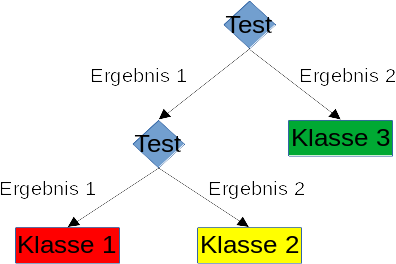
\includegraphics[width=0.5\linewidth]{images/entscheidungsbaum.png}
    \caption{Beispiel eines binären Entscheidungsbaums mit 3 möglichen Ergebnissen.}
    \label{fig:entscheidungsbaum}
\end{figure}
Das Trainieren von Entscheidungsbäumen ist eine Art von \textit{Supervised Learning}, d. h. aus einer beschrifteten Trainingsmenge werden Regeln abgeleitet, um das korrekte Mapping von Input
zu Output abzubilden \cite{goshKMeans}. Die Trainingsmenge besteht aus Feature-Mengen, die mit Klassen beschriftet sind \cite{steinbergCART}. Die Generalisierungsfähigkeit ist abhängig von der
Trainingsmenge. Zum einen sollte die Trainingsmenge möglichst repräsentativ sein für die Aufgabe, die gelernt werden soll. Zum anderen sollten die verwendeten Features eine Partitionierung
aller Klassen ermöglichen \cite{pei1998feature}.
\newline
\newline
Entscheidungsbäume werden heuristisch konstruiert, da die Konstruktion eines optimalen Entscheidungsbaumes NP-Vollständig ist \cite{laurent1976constructing}. Zu diesen Algorithmen gehören
beispielsweise \texttt{ID3} \cite{quinlan1986induction}, \texttt{C4.5} \cite{quinlan2014c4} oder \texttt{CART} \cite{breiman1984classification}. Die Aufgabe ist durch gezielte Trennungen
eine Partitionierung der Trainingsmenge zu erzeugen, sodass möglichst nur Einträge mit der gleichen Beschriftung in einer Partitionierung enthalten sind. Die Algorithmen unterscheiden
sich in ihrer Strategie \cite{quinlan1986induction}.
\newline
\newline
Scikit-Learn implementiert eine optimierte Version des \textit{CART} (\textbf{C}lassification \textbf{A}nd \textbf{R}egression \textbf{T}rees) Algorithmus \cite{ScikitLearnCART}.
CART partitioniert die Trainingsmenge indem lokal immer die beste Teilung ausgewählt wird, d. h. es wird für die momentane Teilmenge immer die beste Teilungsregel ausgewählt.
Dieser Vorgang wird rekursiv mit jeder Teilmenge wiederholt, bis keine weitere Teilung mehr möglich ist oder alle Einträge einer Partitionierung die gleiche Beschriftung tragen \cite{steinbergCART}.
\section{Ensemble-Methoden}
\label{sec:dt_ensemble_methods}
Ensemble-Methoden beschreiben wie mehrere Entscheidungsbäume trainiert werden, um eine möglichst hohe Diversität der einzelnen Entscheidungsbäume zu erzielen. Das Ergebnis eines Ensembles
ist die Aggregation der Ergebnisse der einzelnen Entscheidungsbäume \cite{dietterich2002ensemble}.
\newline
\newline
Der Wahlklassifizierer $H(x) = w_1 h_1(x) + ... + w_K h_K(x)$ ist eine Möglichkeit die Einzelergebnisse $\{h_1, ..., h_K\}$ gewichtet mit $\{w_1, ..., w_K\}$ zu aggregieren \cite{dietterich2002ensemble}.
Ein Ergebnis kann auf zwei Arten modelliert sein.
Einerseits als eine Funktion $h_i: D^n \mapsto \setR^m$, die einer $n$-dimensionalen Menge $D^n$ jeder der $m$ möglichen Klassen eine Wahrscheinlichkeit zuweist.
Das Ergebnis ist eine Wahrscheinlichkeitsverteilung.
Das diskrete Ergebnis der Klassifizierung ist die Klasse mit der höchsten Wahrscheinlichkeit in dem Ergebnis.
Alternativ kann es als eine Funktion $h_i: D^n \mapsto M$ abgebildet werden, die diskret auf eine der möglichen Klassen in $M$ verweist \cite{dymelThesis}.
In diesem Fall wird die Klasse ausgewählt, die am häufigsten unter allen Einzelergebnissen vorkam.
In der Praxis wird die Aggregation der Wahrscheinlichkeitsverteilung genutzt \cite{ScikitLearnEnsemble}.
Analog ist $H: D^n \mapsto \setR^m$ oder $H: D^n \mapsto M$ definiert \cite{dietterich2002ensemble}.
Für gewöhnlich hat jeder Teilnehmer einer Wahl das gleiche Gewicht.
\newline
\newline
Bagging (\textbf{B}ootstrap \textbf{agg}regat\textbf{ing}) konstruiert Entscheidungswälder, indem es Entscheidungsbäume mit Teilmengen der Trainingsmenge trainiert.
Abbildung \ref{fig:bagging} illustriert die Bagging Methode für $n$ Entscheidungsbaummodelle. Zunächst wird die Trainingsmenge in $n$ Teilmengen aufgeteilt \cite{breiman1996bagging}.
Der Inhalt der Teilmengen wird mit der \glqq Bootstrap sampling\grqq\ Methode bestimmt. Diese zieht aus einer Grundmenge $l$-mal jeweils $k$-Einträge \cite{efron1992bootstrap}.
Mit jeder Teilmenge wird ein Entscheidungsbaum trainiert \cite{breiman1996bagging}. Die Einzelergebnisse werden aggregiert, z. B. mit dem Wahlklassifizierer.
\begin{figure}[h!]
    \centering
    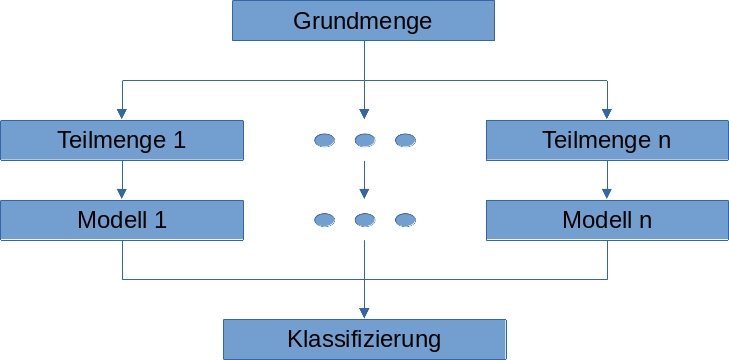
\includegraphics[width=0.6\linewidth]{images/bagging.jpg}
    \caption{Klassifizierungsprozess mit der Bagging-Methode.}
    \label{fig:bagging}
\end{figure}
\newline
\newline
Random Forest erweitert die Bagging-Methode \cite{breiman2001random}. Für jeden Entscheidungsbaum der trainiert werden soll, wird zusätzlich zufällig eine Teilmenge der Feature-Menge ausgewählt.
\newline
\newline
Extremely Randomized Trees (ExtraTrees) verwenden ebenfalls eine Teilmenge der Feature-Menge der Trainingsmenge beim Trainieren der einzelnen Entscheidungsbäume \cite{geurts2006extremely}.
Allerdings wird für jeden Entscheidungsbaum die gesamte Trainingsmenge verwendet. Bei der Konstruktion wird nicht versucht die beste Teilungsregel zu finden,
sondern es werden zufällig Teilungsregeln generiert, aus denen die Beste ausgewählt wird.
\newline
\newline
Beim Boosting werden nacheinander schwache Lerner auf einer Teilmenge trainiert, die gewichtet aggregiert werden \cite{freund1997decision}. Dadurch entsteht ein starker Lerner.
Abbildung \ref{fig:boosting} illustriert, wie vier schwache Lerner trainiert werden. Jeder Lerner findet eine Funktion der die trainierte Teilmenge unterteilt. Anschließend
werden sie gewichtet aggregiert. Dies konstruiert einen starken Lerner, der die gesamte Trainingsmenge unterteilt.
Diese Arbeit verwendet für Boosting den Algorithmus \texttt{AdaBoost} \cite{freund1997decision} von Freund und Schapire.
\begin{figure}[h!]
    \centering
    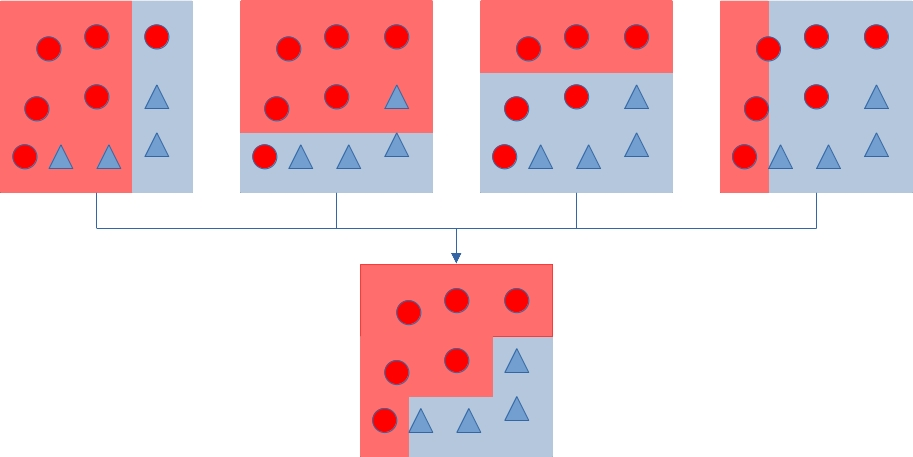
\includegraphics[width=\linewidth]{images/boosting.jpg}
    \caption{Klassifizierungsprozess mit der Boosting-Methode.}
    \label{fig:boosting}
\end{figure}
\section{Cherry-Picking}
\begin{itemize}
    \item Gehe hier auf Monte Carlo etc ein.
\end{itemize}
\section{Ressourcenbedarf auf dem Mikrocontroller}
\label{sec:dt_resource_usage}
Zukünftig soll das Modell auf einem Mikrocontroller ausgeführt werden \cite{antragForschungsprojekt}.
Mikrocontroller sind stark limitiert in ihrer Rechenleistung, Speicherkapazität, RAM und werden oft zudem mit einer Batterie betrieben.
Aus diesem Grund ist der Energieverbrauch zu minimieren und das Modell muss innerhalb dieser Limitierungen operieren können.

\newpage
\subsection{Ausführungszeit und Energieverbrauch}
\label{sub_sec:dt_ru_execution_time}
Der Energieverbrauch korreliert mit der Ausführungszeit.
Je länger die CPU ausgeschaltet ist, desto weniger Energie wird verbraucht.
Kurze Ausführungszeiträume vergrößern den Zeitraum, in dem die CPU ausgeschaltet sein kann.
Die Ausführungszeit ist die Zeit die benötigt wird, um alle Instruktionen auszuführen \cite{dymelThesis}.
Jede Instruktion bedarf eine bestimmte Anzahl an CPU-Zyklen.
Die Zeit pro Zyklus ist abhängig von der Taktrate der CPU.
\newline
\newline
Die Ausführungszeit eines Entscheidungswaldes setzt sich zusammen aus der Zeit für die Feature-Extrahierung, der Evaluierung aller im Ensemble enthaltenen Entscheidungsbäume
und der Aggregierungsfunktion.
Im schlimmsten Fall muss die gesamte Höhe eines Entscheidungsbaumes traversiert werden, um das Ergebnis zu bestimmen. Aus diesem Grund skaliert die Ausführungszeit mit der
traversierten Höhe jedes Baumes.
\newline
\newline
Um die Instruktionen zu minimieren sollten Datentypen verwendet werden, die von der CPU mit höchstens einem Wort dargestellt werden können.
Eine 8-Bit CPU würde zum Laden in Register eines 32-Bit Datentypen vier mal so viele Instruktionen benötigen wie bei einem 8-Bit Datentypen.
Außerdem sollten Operationen verwendet werden, die durch native Hardware-Operationen abgebildet werden können.
Ist dem nicht so, muss diese Operation durch Software ersetzt werden.
Dies erfordert mehr Zyklen als eine native Operation in Hardware.
\newline
\newline
Zu Beachten bei der Minimierung ist, dass Instruktionen unterschiedlich viele Zyklen benötigen und Funktionsaufrufe Overhead erzeugen.
Ein Beispiel dafür ist die Optimierung \textit{Function Inlining} \cite{leupers1999function}.
Der Aufruf von Funktionen kann einen hohen Overhead durch den Kontextwechsel erzeugen.
Aus diesem Grund verringert diese Optimierung die Ausführungszeit, erhöht aber die die Programmgröße signifikant.
Im Umkehrschluss könnten durch die Verwendung von Funktionen der nutzen des Programmspeichers verringert werden, Ausführungszeit und Energieverbrauch aber erhöht werden.

\newpage
\subsection{Programmgröße}
\label{sub_sec:dt_ru_programm_size}
Die Programmgröße ist die Gesamtheit aller Instruktionen die für das Programm benötigt werden \cite{dymelThesis}.
Dabei ist der Anteil für die Entscheidungswälder integral und der Anteil für die perifären Funktionalitäten zu vernachlässigen.
Die Programmgröße, die für einen Entscheidungswald benötigt wird, skaliert mit der Waldgröße und Höhe der einzelnen Entscheidungsbäume.
\newline
\newline
Die Höhe des Entscheidungsbaumes ist die Verzweigungstiefe der verschachtelten Tests.
Jeder Test ist ein Vergleich mit einem Schwellenwert.
Die Programmgröße für einen Vergleich setzt sich zusammen aus den Operationen um die Operanden in die Register zu laden
und die Instruktion um den Vergleich durchzuführen, sowie Abzweiginstruktionen. Wie in Kapitel \ref{sub_sec:dt_ru_execution_time}
sind Instruktionen durch einen passenden Datentypen zu vermeiden.
\newline
\newline
Ein weiterer Faktor sind die Instruktionen, die zur Rückgabe des Klassifizierungsergebnis benötigt werden.
In Kapitel \ref{sec:dt_ensemble_methods} wurden verschiedene Möglichkeiten der Rückgabe diskutiert, die relevant bei dem Aggregierungsprozess eines Ensembles ist.
Einerseits kann die Rückgabe eine Wahrscheinlichkeitsverteilung sein und andererseits eine diskrete Klasse.
Bei $m$ möglichen Klassen würde die erste Variante $m$-mal so viele Instruktion benötigen, wie die zweite Variante, da der Rückgabevektor zuvor mit der Wahrscheinlichkeitsverteilung gefüllt werden muss.
In der Praxis werden aber weniger Instruktion benötigt, da es eine große Überschneidung der Wahrscheinlichkeitsverteilungen gibt, die zurück gegeben werden.
Die Instruktionen, um den Rückgabevektor zu befüllen, können durch \textit{Basic Blocks}, d. h. beschriftete Instruktionsblöcke, geschickt recycled werden.
Zudem können Zuweisungen ausgelassen werden, die die Wahrscheinlichkeit 0 zuweisen, da der Vektor mit Nullen initialisiert wird.
Dennoch werden signifikant mehr Instruktionen benötigt als bei der diskreten Variante.
Aus diesem Grund wurde ein hybrider Ansatz vorgeschlagen, der im Falle eines eindeutigen Ergebnisses mit einer Toleranz von $\epsilon\in [0, 1]$ die diskrete Klasse statt der Wahrscheinlichkeitsverteilung zurück gibt.
